\documentclass{article}

\usepackage{graphicx}
\usepackage{tikz}
\usepackage{tikzsymbols}
\usetikzlibrary{calc,patterns,shapes.geometric}
\pagestyle{empty}
\usepackage[margin=0pt]{geometry}
\geometry{papersize={14in,12in}}

\def\centerarc[#1](#2)(#3:#4:#5){\draw[#1] ($(#2)+({#5*cos(#3)},{#5*sin(#3)})$) arc (#3:#4:#5);}

\begin{document}
	\begin{figure}
		\centering
		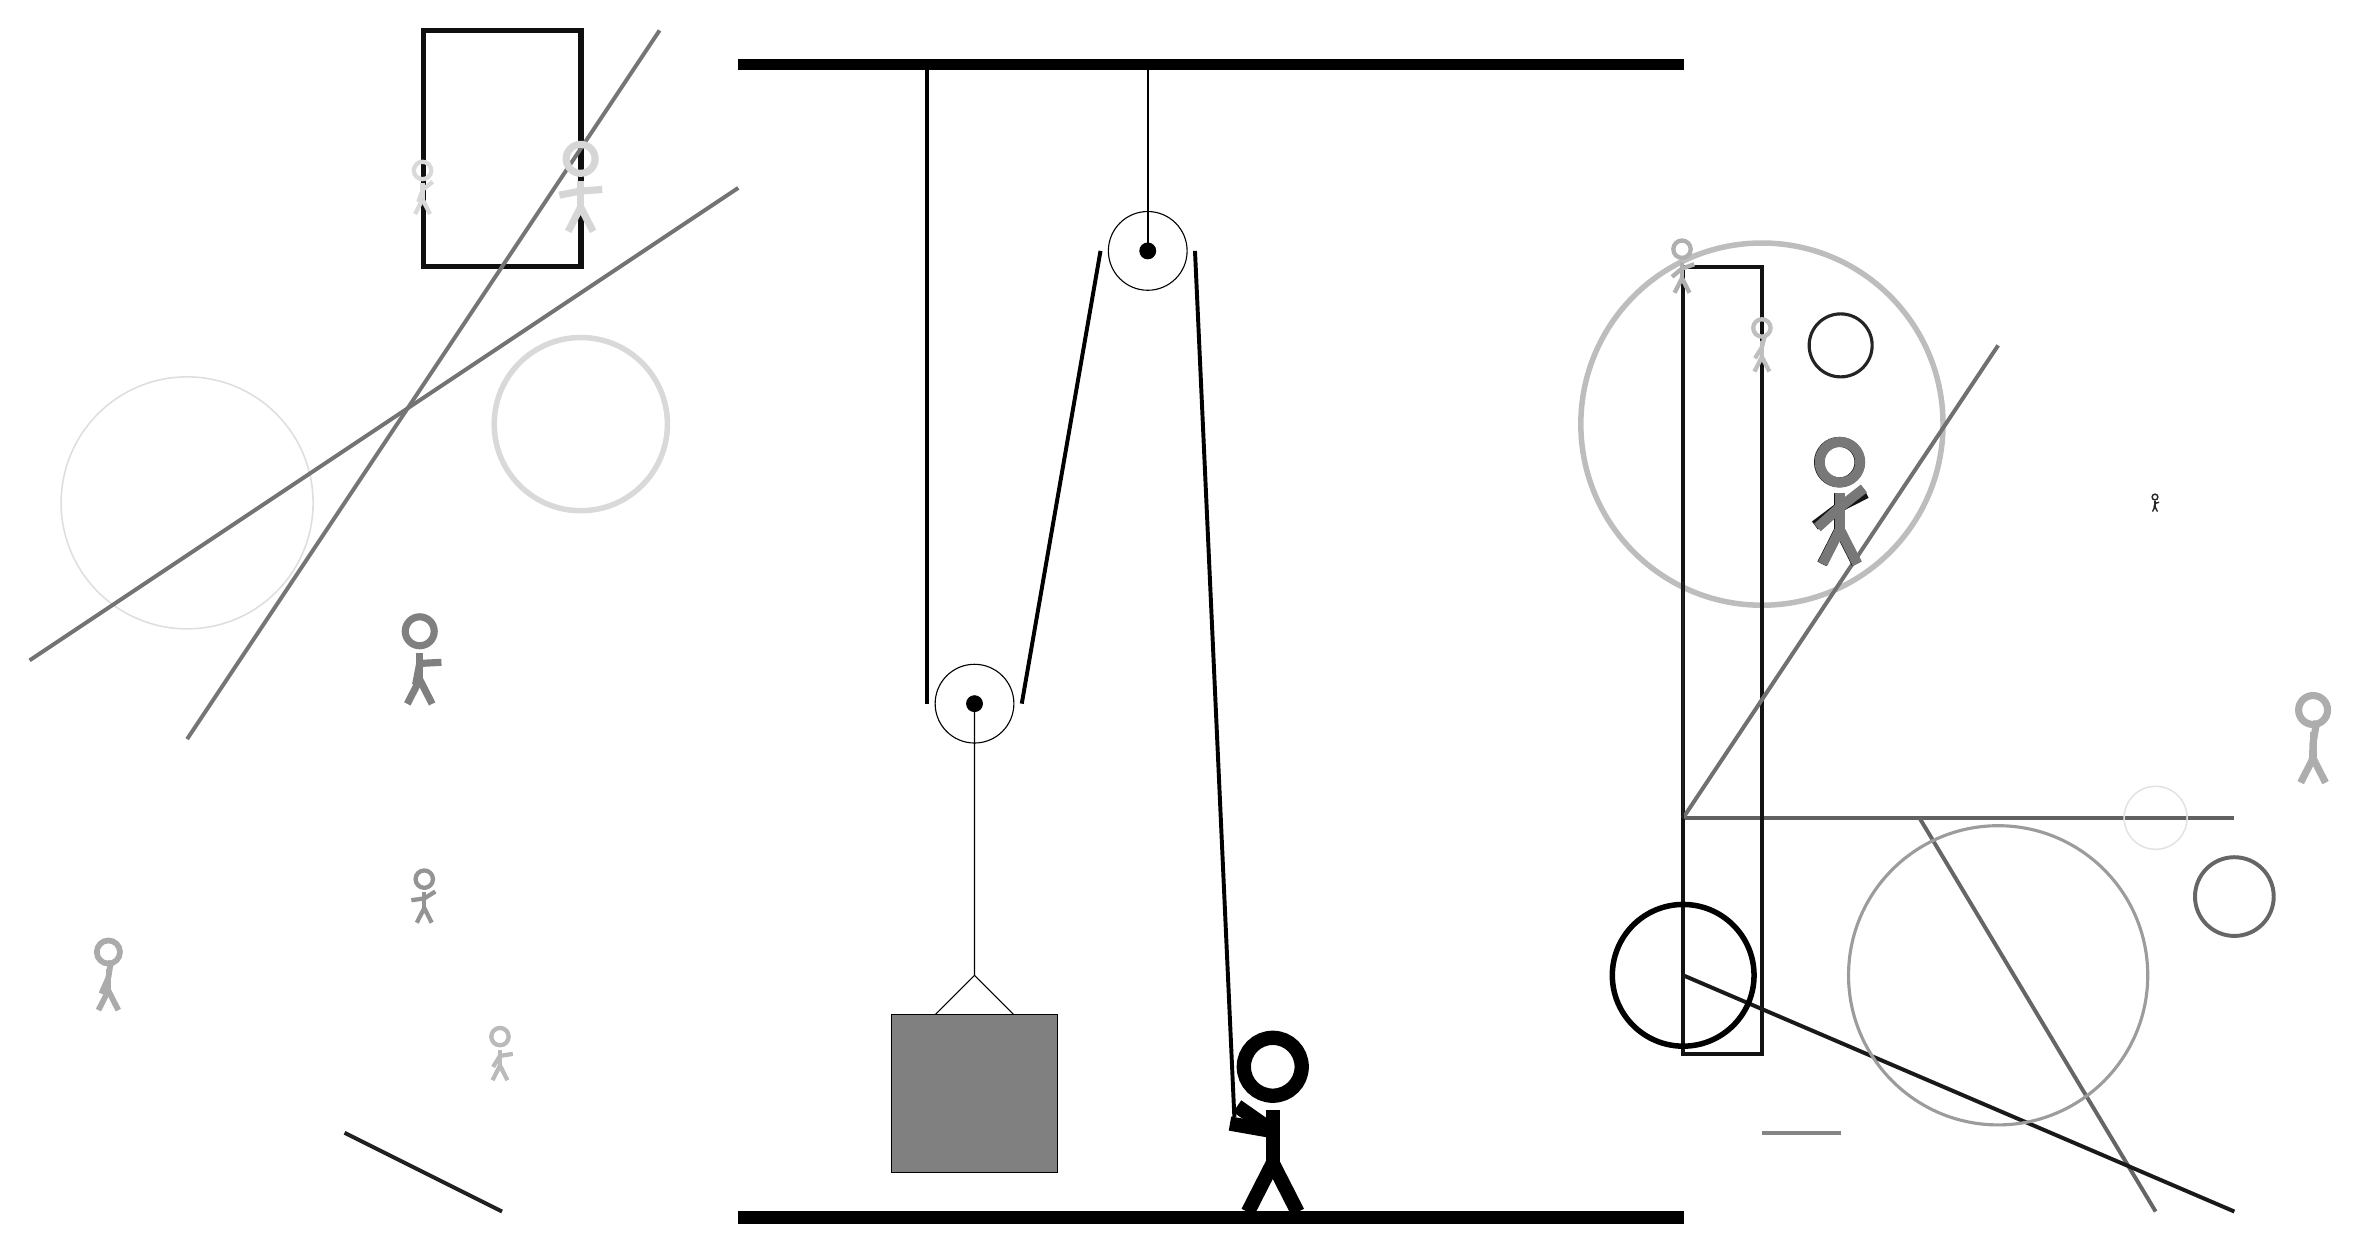
\begin{tikzpicture}
			%%%%% START %%%%%
			
			\draw[fill=black] (-2, 11.5) rectangle (10, 11.625);
			
			\draw [line width=0.7mm, color=black!26](11, 7) circle (2.3);
			
			\draw[line width=0.5mm, color=black!62](10, 2) -- (17, 2);
			\draw[line width=0.5mm, color=black!93] (11, 9) rectangle (10, -1);
			\draw[line width=0.5mm, color=black!56](14, 8) -- (10, 2);
			
			\draw[line width=0.5mm, color=black!48](11, -2) -- (12, -2);
			
			\draw [line width=0.2mm, color=black!11](16, 2) circle (0.4);
			\node[line width=0.2mm, color=black!27] at (-5, -1) {\Strichmaxerl[3][58][9]};
			\draw[line width=0.7mm, color=black!94] (-4, 9) rectangle (-6, 12);
			\draw[line width=0.5mm, color=black!60](13, 2) -- (16, -3);
			
			\draw[line width=0.2mm, color=black!87] (10, 5) rectangle (10, 2);
			\draw[line width=0.5mm, color=black!90](10, 0) -- (17, -3);
			\node[line width=0.6mm, color=black!92] at (12, 6) {\Strichmaxerl[7][37][27]};
			\draw [line width=0.4mm, color=black!39](14, 0) circle (1.9);
			\node[line width=0.2mm, color=black!33] at (-10, 0) {\Strichmaxerl[4][66][81]};
			\node[line width=0.6mm, color=black!31] at (10, 9) {\Strichmaxerl[3][40][19]};
			\node[line width=0.3mm, color=black!25] at (11, 8) {\Strichmaxerl[3][58][76]};
			
			\draw [line width=0.4mm, color=black!86](12, 8) circle (0.4);
			\node[line width=0.3mm, color=black!50] at (-6, 4) {\Strichmaxerl[5][79][3]};
			\draw[line width=0.5mm, color=black!87](-5, -3) -- (-7, -2);
			\draw [line width=0.7mm, color=black!15](-4, 7) circle (1.1);
			\draw [line width=0.5mm, color=black!60](17, 1) circle (0.5);
			
			\node[line width=0.4mm, color=black!32] at (18, 3) {\Strichmaxerl[5][88][80]};
			\node[line width=0.6mm, color=black!85] at (16, 6) {\Strichmaxerl[1][76][17]};
			\draw [line width=0.2mm, color=black!13](-9, 6) circle (1.6);
			\draw[line width=0.5mm, color=black!54](-3, 12) -- (-9, 3);
			
			\node[line width=0.6mm, color=black!53] at (12, 6) {\Strichmaxerl[7][42][38]};
			
			\node[line width=0.4mm, color=black!42] at (-6, 1) {\Strichmaxerl[3][8][32]};
			\node[line width=0.3mm, color=black!15] at (-6, 10) {\Strichmaxerl[3][71][38]};
			\draw [line width=0.7mm, color=black!100](10, 0) circle (0.9);
			\draw[line width=0.5mm, color=black!55](-2, 10) -- (-11, 4);
			\node[line width=0.6mm, color=black!16] at (-4, 10) {\Strichmaxerl[5][11][4]};
			
			\draw (3.2, 9.2) circle (0.5);
			\draw[fill=black] (3.2, 9.2) circle (0.1);
			\draw[thick] (3.2, 9.2) -- (3.2, 11.5);
			
			\draw (1, 3.45) circle (0.5);
			\draw[fill=black] (1, 3.45) circle (0.1);
			
			\draw (1, 3.45) -- (1, 0.0) -- (0.5, -0.5);
			\draw (1, 0.0) -- (1.5, -0.5);
			\draw[fill=black!50] (-0.05, -0.5) rectangle (2.05, -2.5);
			
			\draw[line width=0.5mm] (0.4, 11.5) -- (0.4, 3.45);
			\centerarc[line width=0.5mm](1, 3.45)(180:360:0.6);
			\draw[line width=0.5mm](1.6, 3.45) -- (2.6, 9.2);
			\centerarc[line width=0.5mm](3.2, 9.2)(0:180:0.6);
			\draw[line width=0.5mm](3.8, 9.2) -- (4.3, -1.8);
			
			\node at (4.7, -1.9) {\Strichmaxerl[10][-35][170]};
			
			\draw[fill=black] (-2, -3) rectangle (10, -3.15);
			
			%%%%% END %%%%%
		\end{tikzpicture}
	\end{figure}	
\end{document}